\documentclass[english,11pt]{beamer}

\DeclareMathOperator{\Cov}{Cov}
\DeclareMathOperator{\Var}{Var}
\DeclareMathOperator{\E}{\mathbb{E}}
\DeclareMathOperator{\Proba}{\mathbb{P}}

\newcommand{\Covb}[2]{\ensuremath{\Cov\!\left[#1,#2\right]}}
\newcommand{\Eb}[1]{\ensuremath{\E\!\left[#1\right]}}
\newcommand{\Pb}[1]{\ensuremath{\Proba\!\left[#1\right]}}
\newcommand{\Varb}[1]{\ensuremath{\Var\!\left[#1\right]}}

% norm
\newcommand{\norm}[1]{\| #1 \|}

\newcommand{\indep}{\rotatebox[origin=c]{90}{$\models$}}





\usepackage{mathptmx,amsmath,amssymb,graphicx,bibentry,bbm,babel,ragged2e}

\makeatletter

\newcommand{\noun}[1]{\textsc{#1}}
\newcommand{\jitem}[1]{\item \begin{justify} #1 \end{justify} \vfill{}}
\newcommand{\sframe}[2]{\frame{\frametitle{#1} #2}}

\newenvironment{centercolumns}{\begin{columns}[c]}{\end{columns}}
%\newenvironment{jitem}{\begin{justify}\begin{itemize}}{\end{itemize}\end{justify}}

\usetheme{Warsaw}
\setbeamertemplate{footline}[text line]{}
\setbeamercolor{structure}{fg=purple!50!blue, bg=purple!50!blue}

\setbeamersize{text margin left=15pt,text margin right=15pt}

\setbeamercovered{transparent}


\@ifundefined{showcaptionsetup}{}{%
 \PassOptionsToPackage{caption=false}{subfig}}
\usepackage{subfig}

\usepackage[utf8]{inputenc}
\usepackage[T1]{fontenc}



\makeatother

\begin{document}


\title{Modeling the Co-evolution of Urban Form and Transportation Networks}

\author{J.~Raimbault$^{1,2,\ast}$\\
\texttt{juste.raimbault@polytechnique.edu}
}


\institute{$^{1}$UMR CNRS 8504 G{\'e}ographie-cit{\'e}s\\
$^{2}$UMR-T IFSTTAR 9403 LVMT
}


\date{Sageo 2017 - Rouen\\\smallskip
November 7th 2017
}

\frame{\maketitle}





%%%%%%%%%%%%%%%%%%%
%% ABSTRACT

%\keywords{Spatio-temporal Causality ; Network-territories Interactions ; Urban Morphogenesis ; Greater Paris}
%This paper contributes to the understanding of strongly coupled spatio-temporal processes by describing a generic method based on Granger causality. The method is validated by the robust identification of causality regimes and of their phase diagram for an urban morphogenesis model that couples network growth with density. The application to the real case study of Greater Paris transportation projects shows a link between territorial dynamics, more particularly of real estate and socio-economic, and the anticipated network growth. We finally discuss potential extensions to other temporal and spatial scales.



%%%%%%%%%%%%%%%%%
\section{Introduction}
%%%%%%%%%%%%%%%%%



\sframe{Circular Causalities in Complex Systems}{

\centering

% striking image

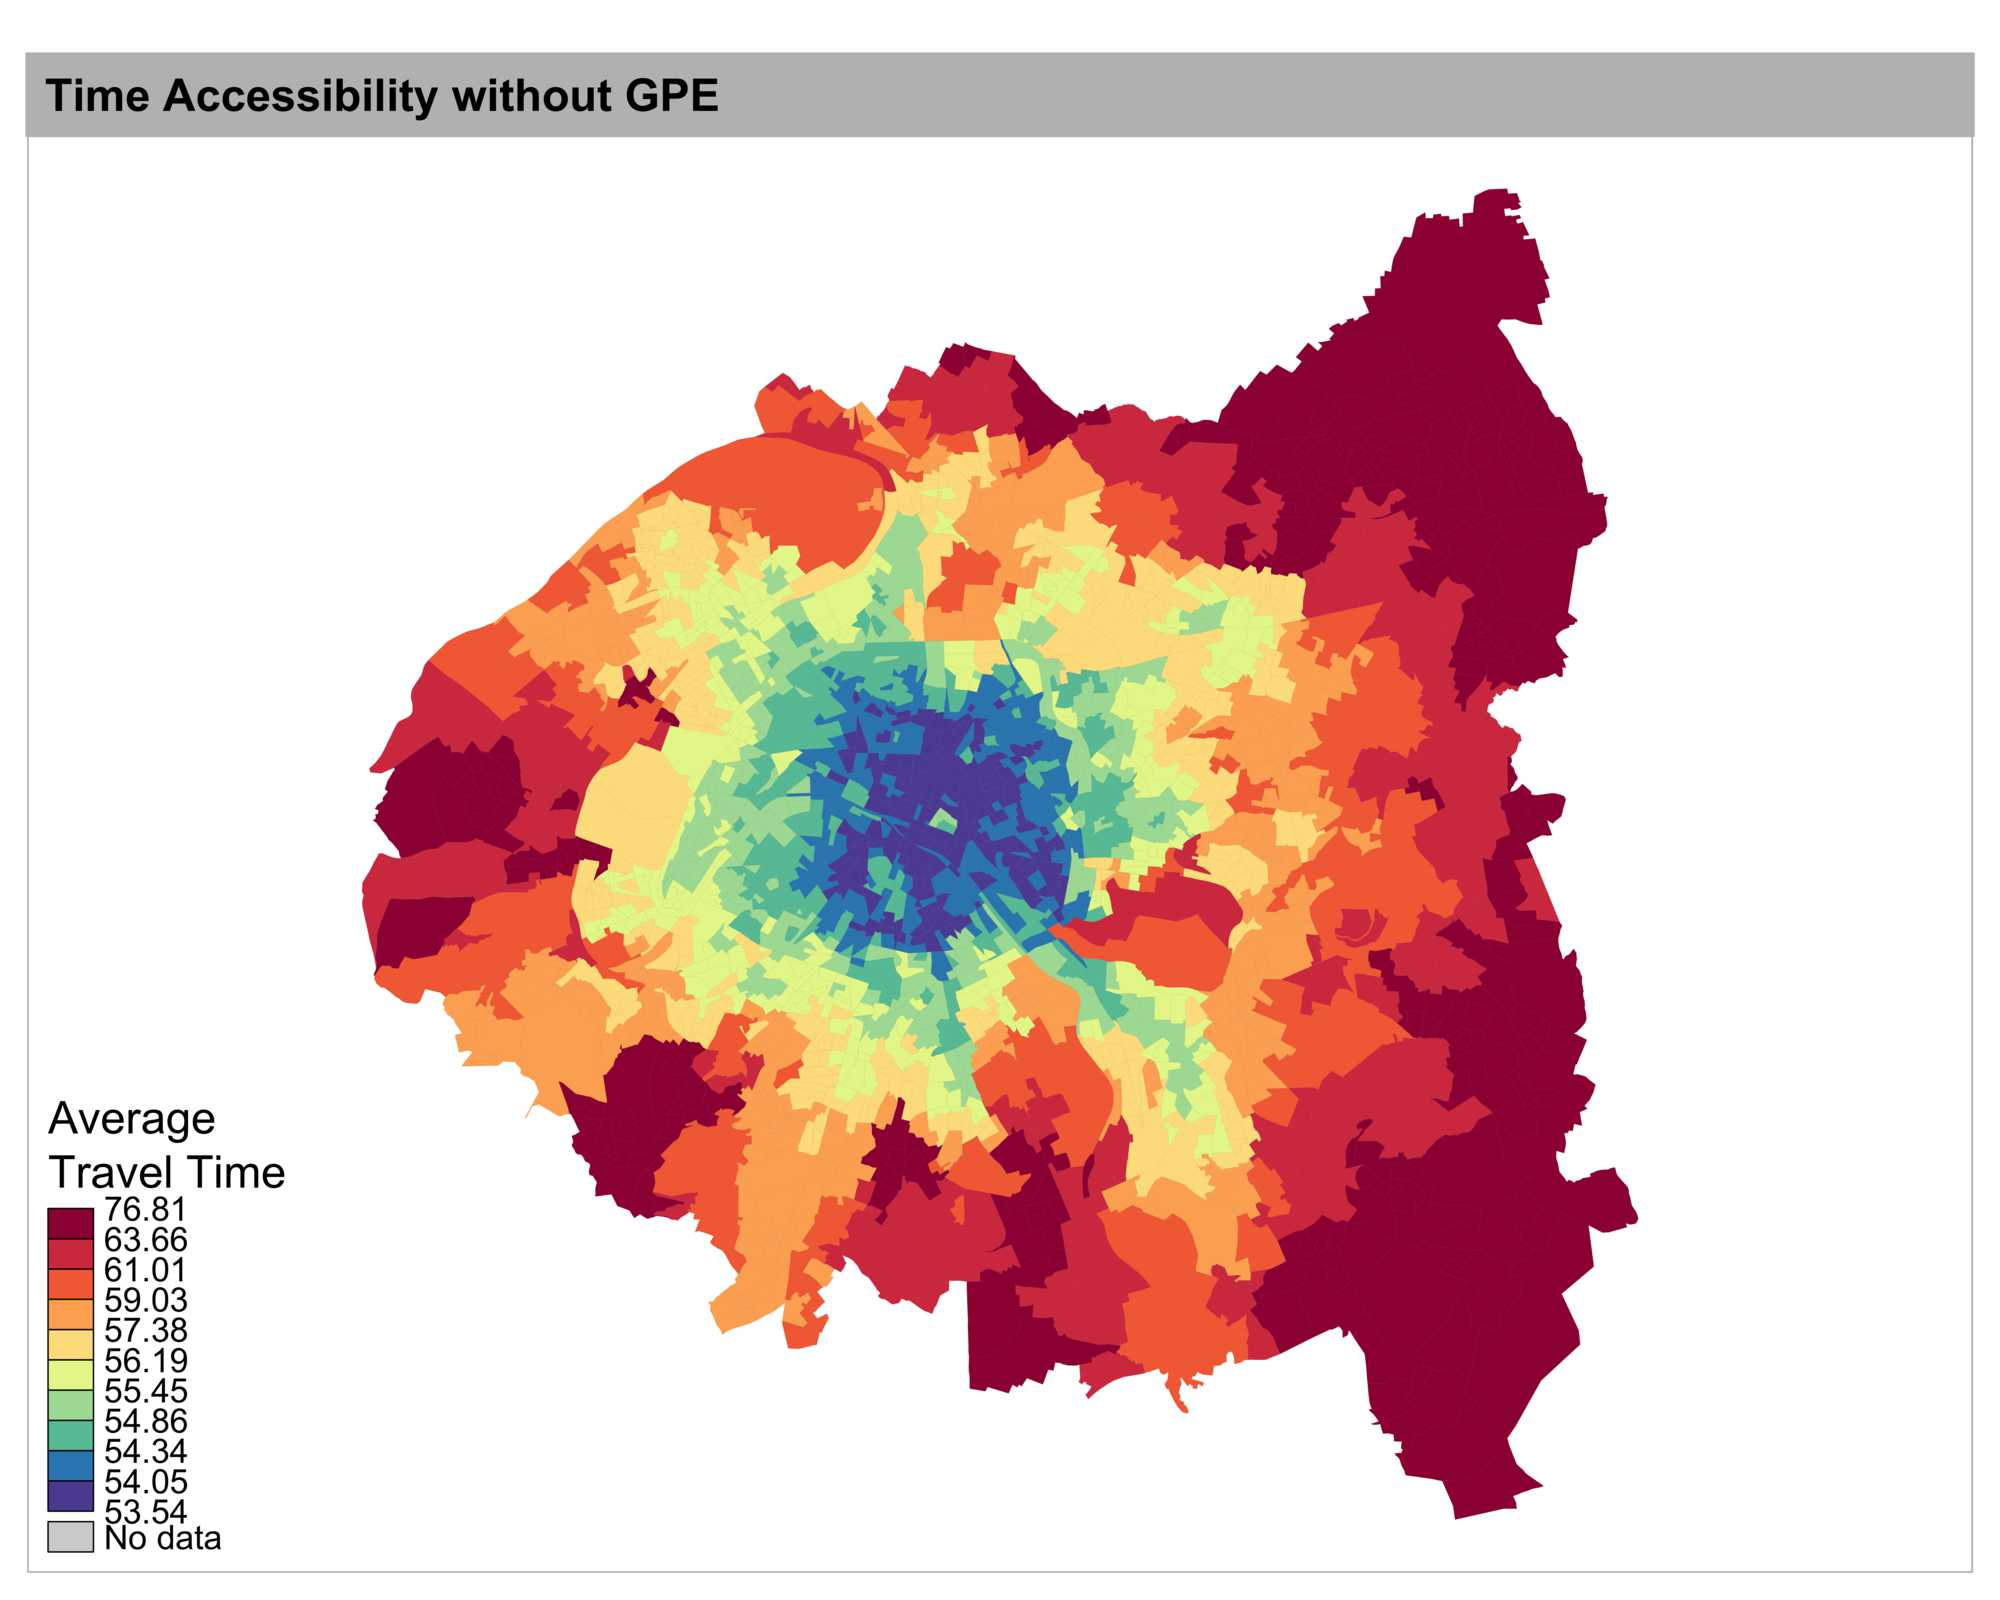
\includegraphics[width=0.48\textwidth]{figures/timeaccess_metropole}
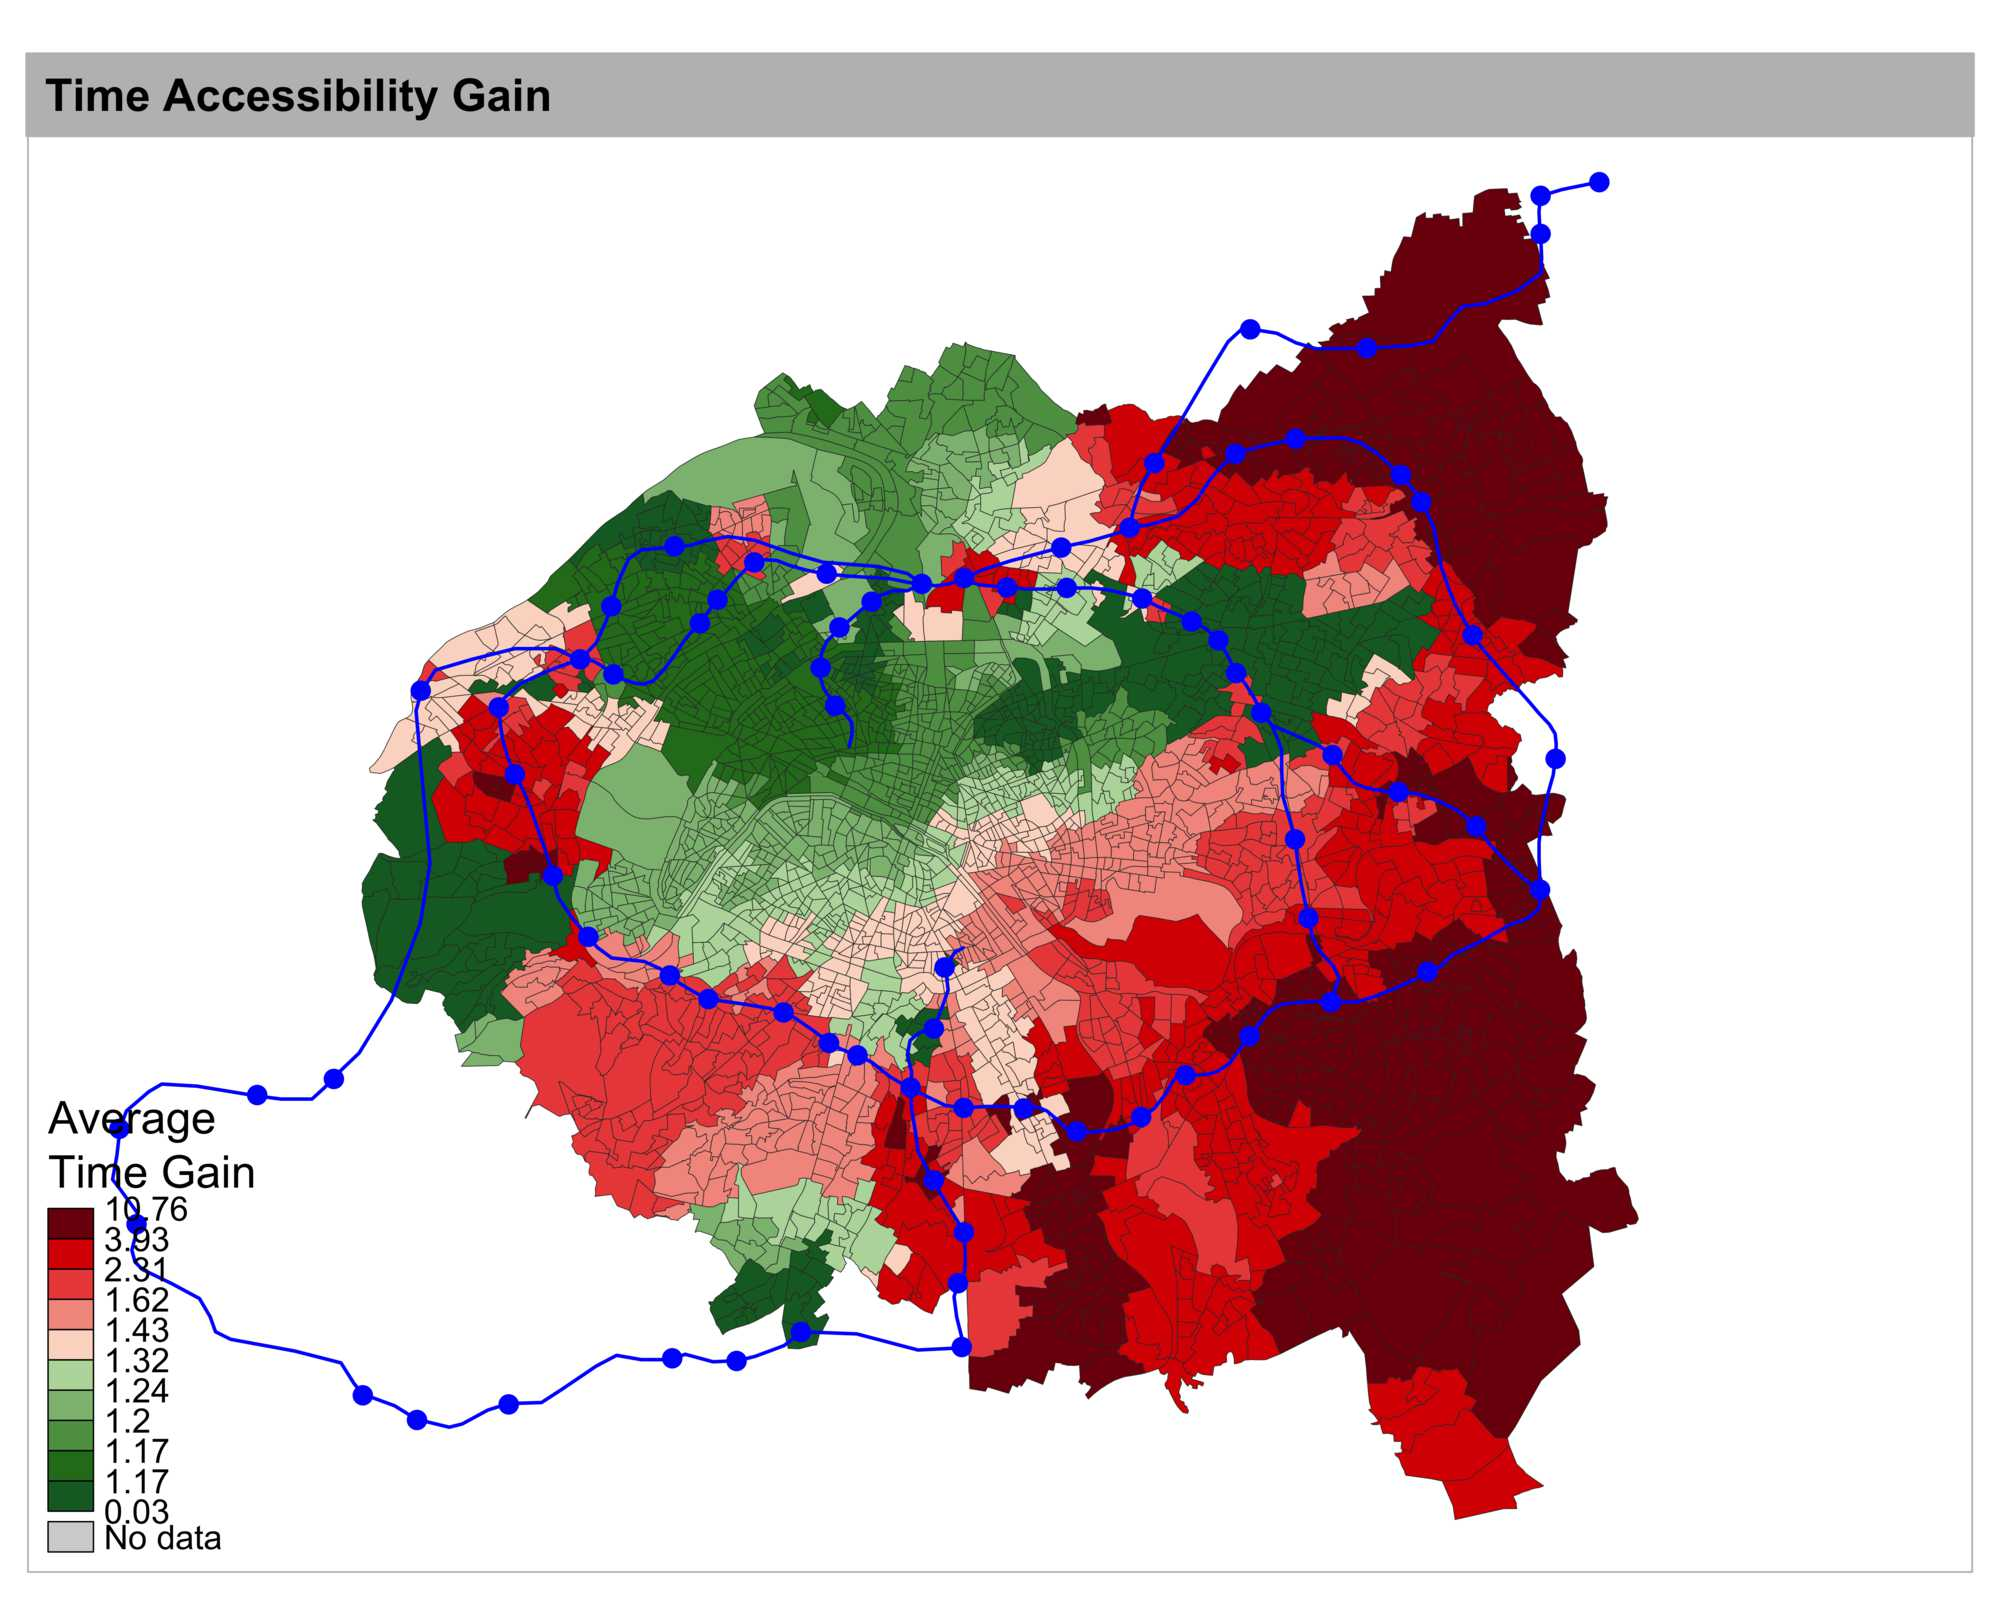
\includegraphics[width=0.48\textwidth]{figures/timegain_metropole}

\textit{Time accessibility gain allowed by GPE new lines}

}


\sframe{Causality in Geography}{


}

\sframe{Existing approaches}{


}

\sframe{Research objective}{

% insist on datamining approach - because Granger causality seen and reseen : structure of data/unsupervised

}





%%%%%%%%%%%%%%%%%
\section{Methods and Results}
%%%%%%%%%%%%%%%%%


\sframe{Method: Rationale}{

}


\sframe{Method: Formalization}{

Correlation estimator $\hat{\rho}$ applying in time, space and repetitions, i.e. $\hat{\rho}\left[X,Y\right] = \hat{\mathbb{E}}_{i,t,k}\left[XY\right] - \hat{\mathbb{E}}_{i,t,k}\left[X\right]\hat{\mathbb{E}}_{i,t,k}\left[Y\right]$

\bigskip

Lagged Correlation

\begin{equation}
\rho_{\tau}\left[X_{j_1},X_{j_2}\right] = \hat{\rho}\left[x^{(k)}_{i,j_1,t - \tau},x^{(k)}_{i,j_2,t}\right]
\end{equation}


}

\sframe{Validation: Synthetic Data}{

% present strategy and rbd model

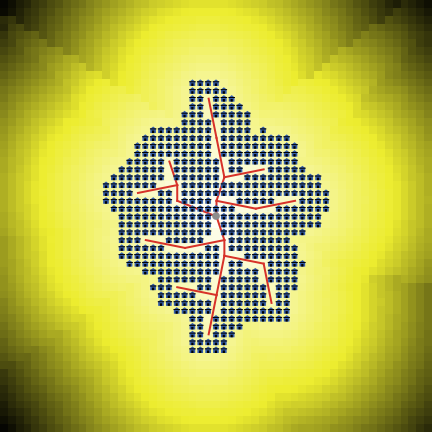
\includegraphics[width=0.32\textwidth]{figures/ex_60_wdens0_wroad1_wcenter1_seed272727}\hspace{0.1cm}
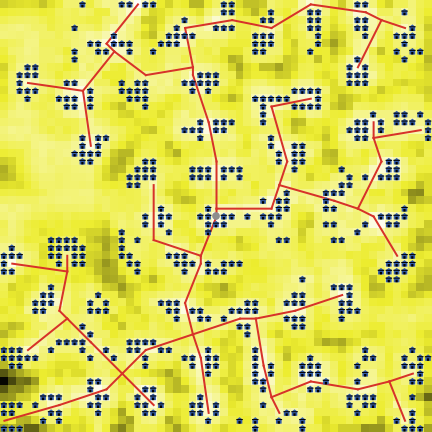
\includegraphics[width=0.32\textwidth]{figures/ex_60_wdens1_wroad1_wcenter0_seed272727}\hspace{0.1cm}
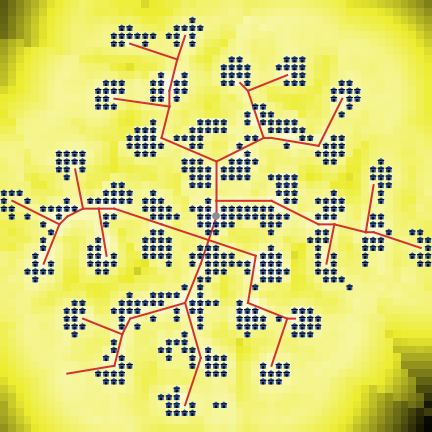
\includegraphics[width=0.32\textwidth]{figures/ex_60_wdens1_wroad1_wcenter1_seed272727}\hspace{0.1cm}

\medskip

\textit{Synthetic urban configurations generated by an hybrid morphogenesis model from \cite{raimbault2014hybrid}}

}

\sframe{Profiles of lagged correlations}{

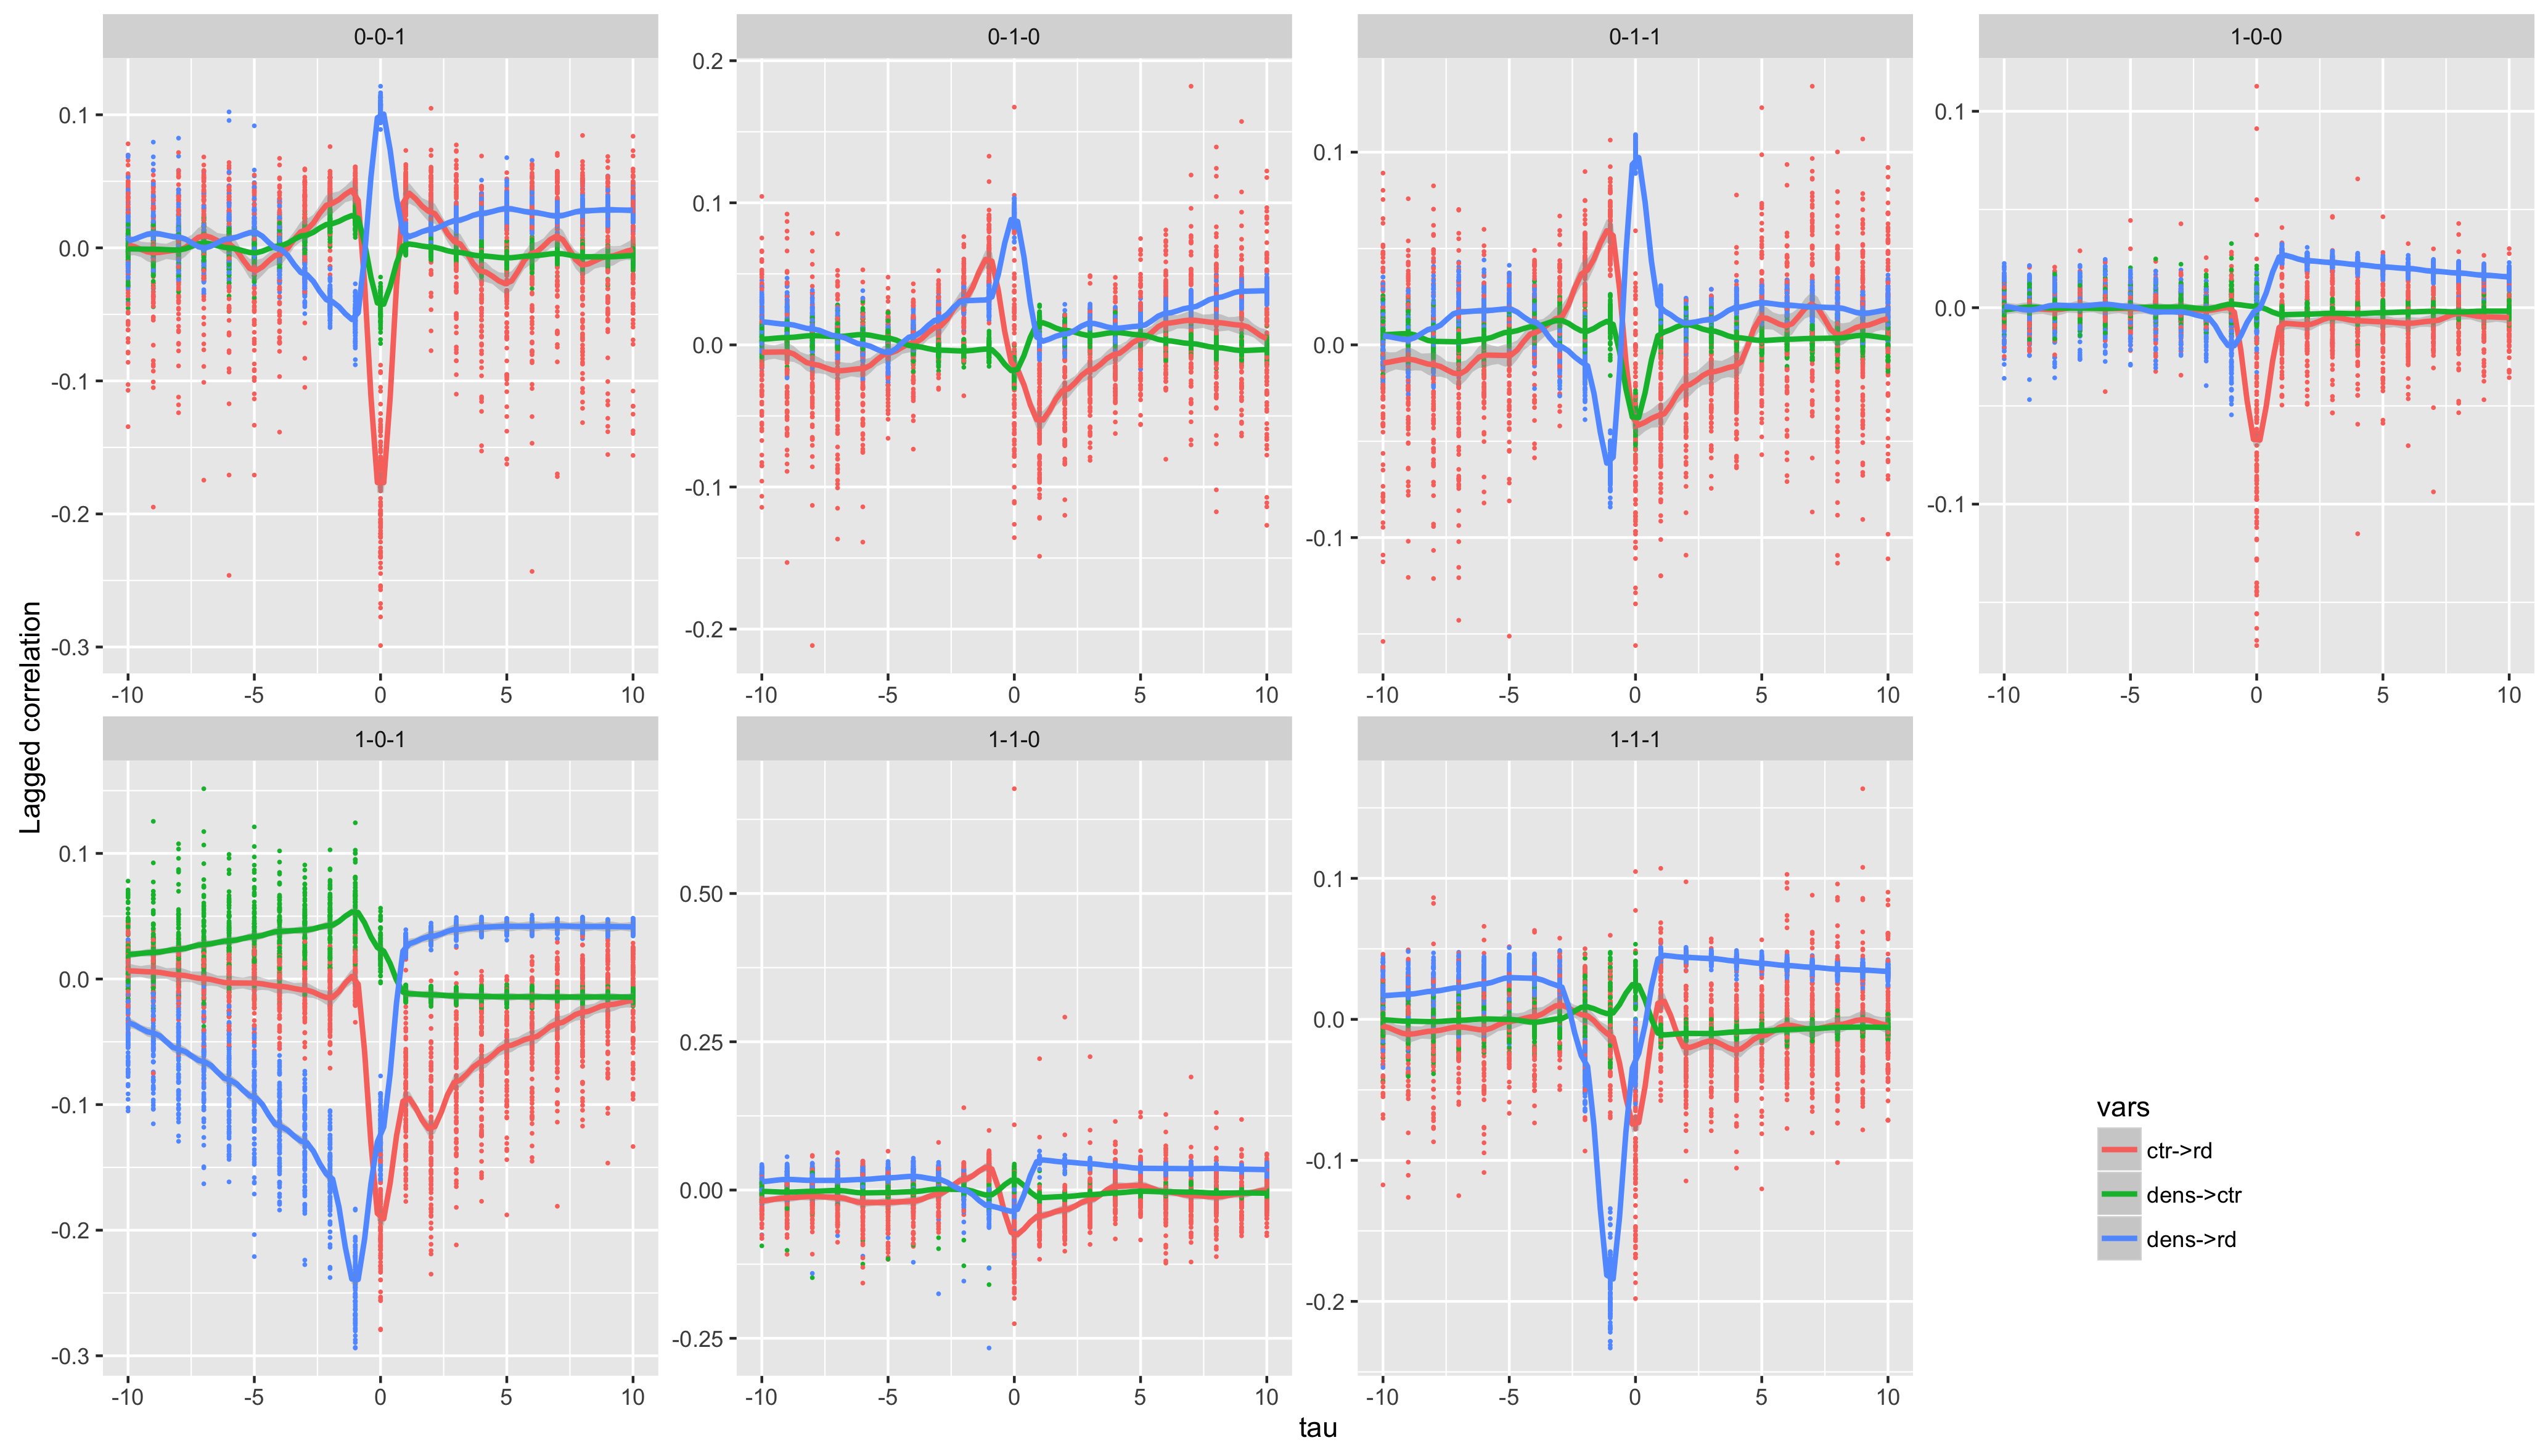
\includegraphics[width=\textwidth]{figures/laggedcorrs_facetextreme}

\medskip

\vspace{-0.2cm}

\textit{Values of $\rho_{\tau}$ for all couples of three explicative variables (density, distance to center, distance to roads), for 8 extreme parameter points}

}


\sframe{Unveiling Endogenous causality regimes}{

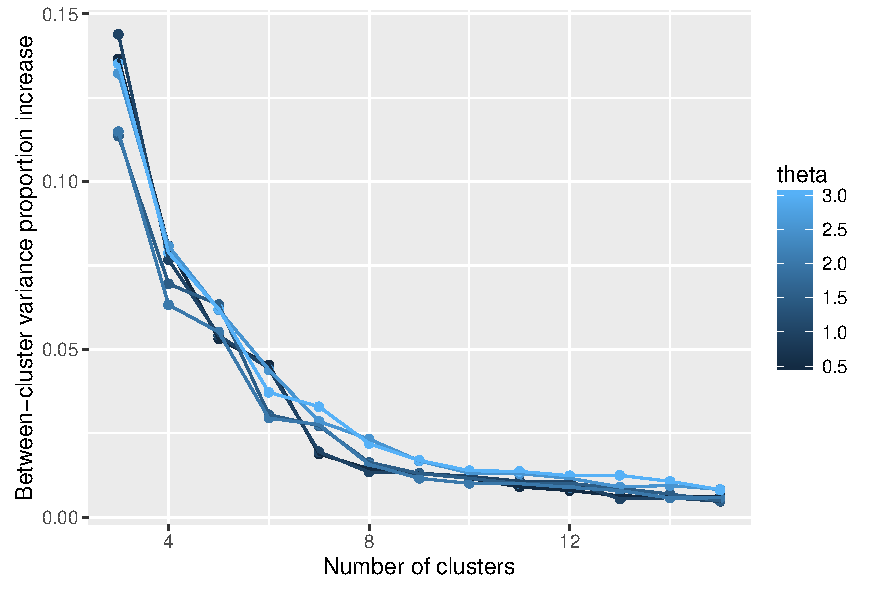
\includegraphics[width=0.48\textwidth]{figures/dccoef-knum_valuesFALSEtheta05-3}
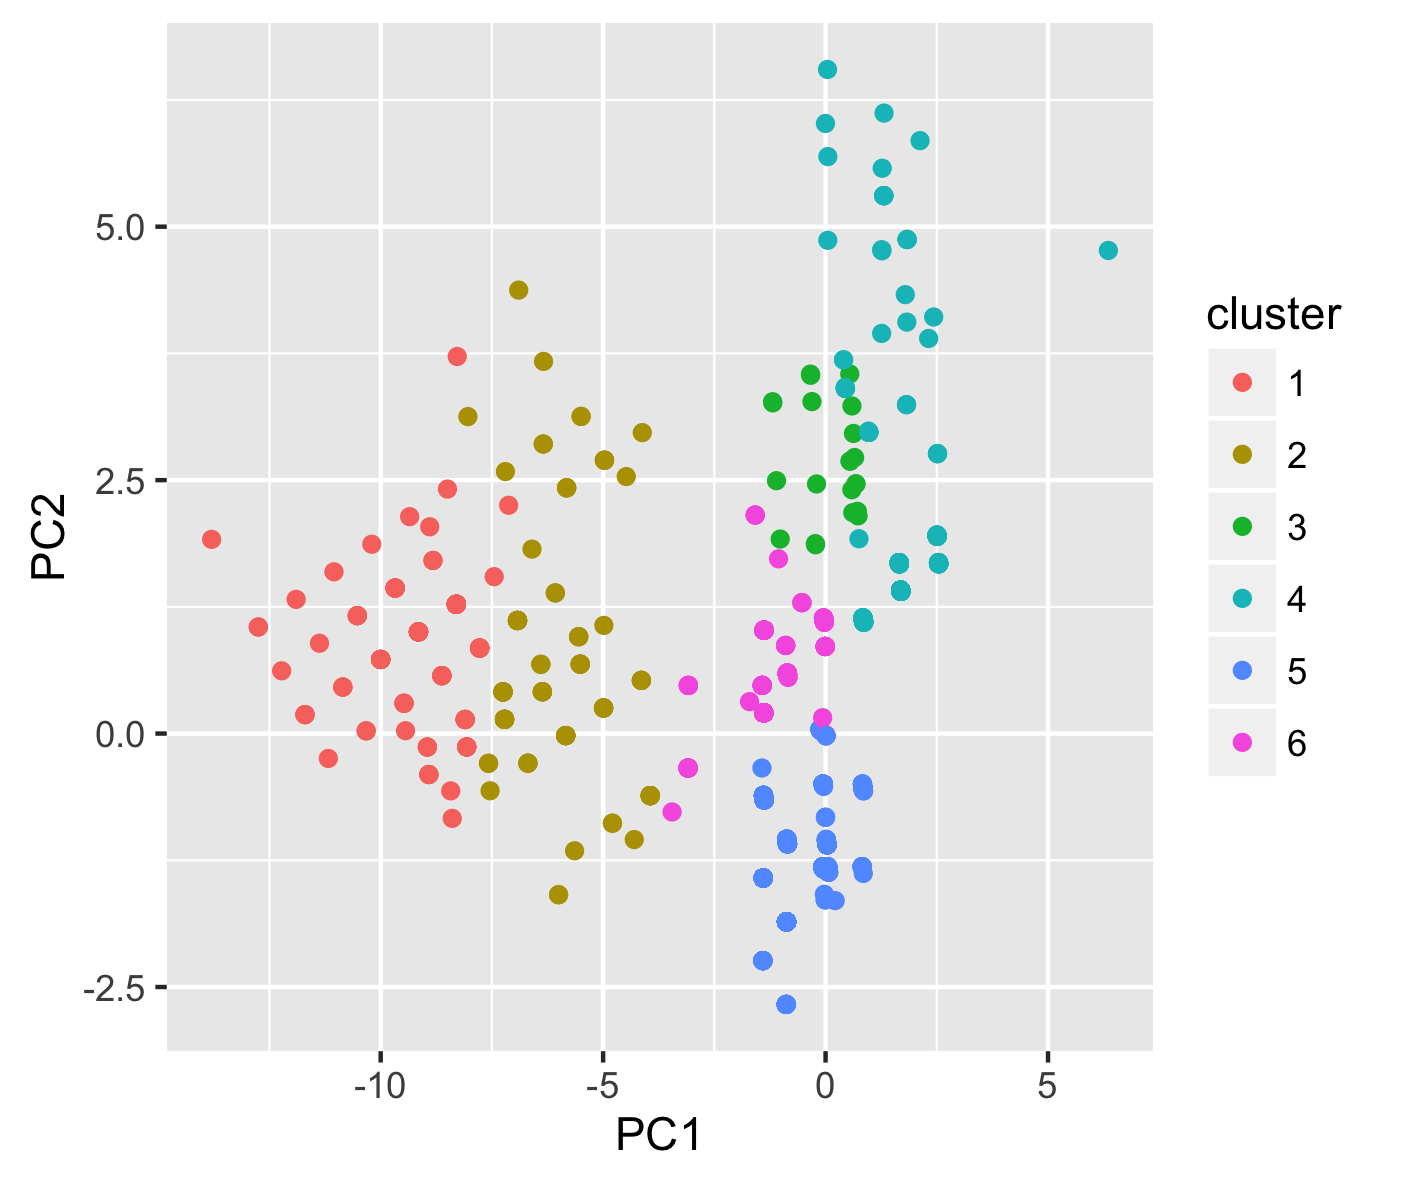
\includegraphics[width=0.48\textwidth]{figures/clusters-PCA-features_valuesFALSEtheta2_k6}

\textit{Unsupervised classification (robust k-means) on $\tau_{min},\tau_{max}$ features: (Left) Derivative of clustering coefficient for number of clusters $k$; (Right) PCA visualisation of classification for ``optimal'' $k$}

}

\sframe{Consistence and interpretation of regimes}{

\centering

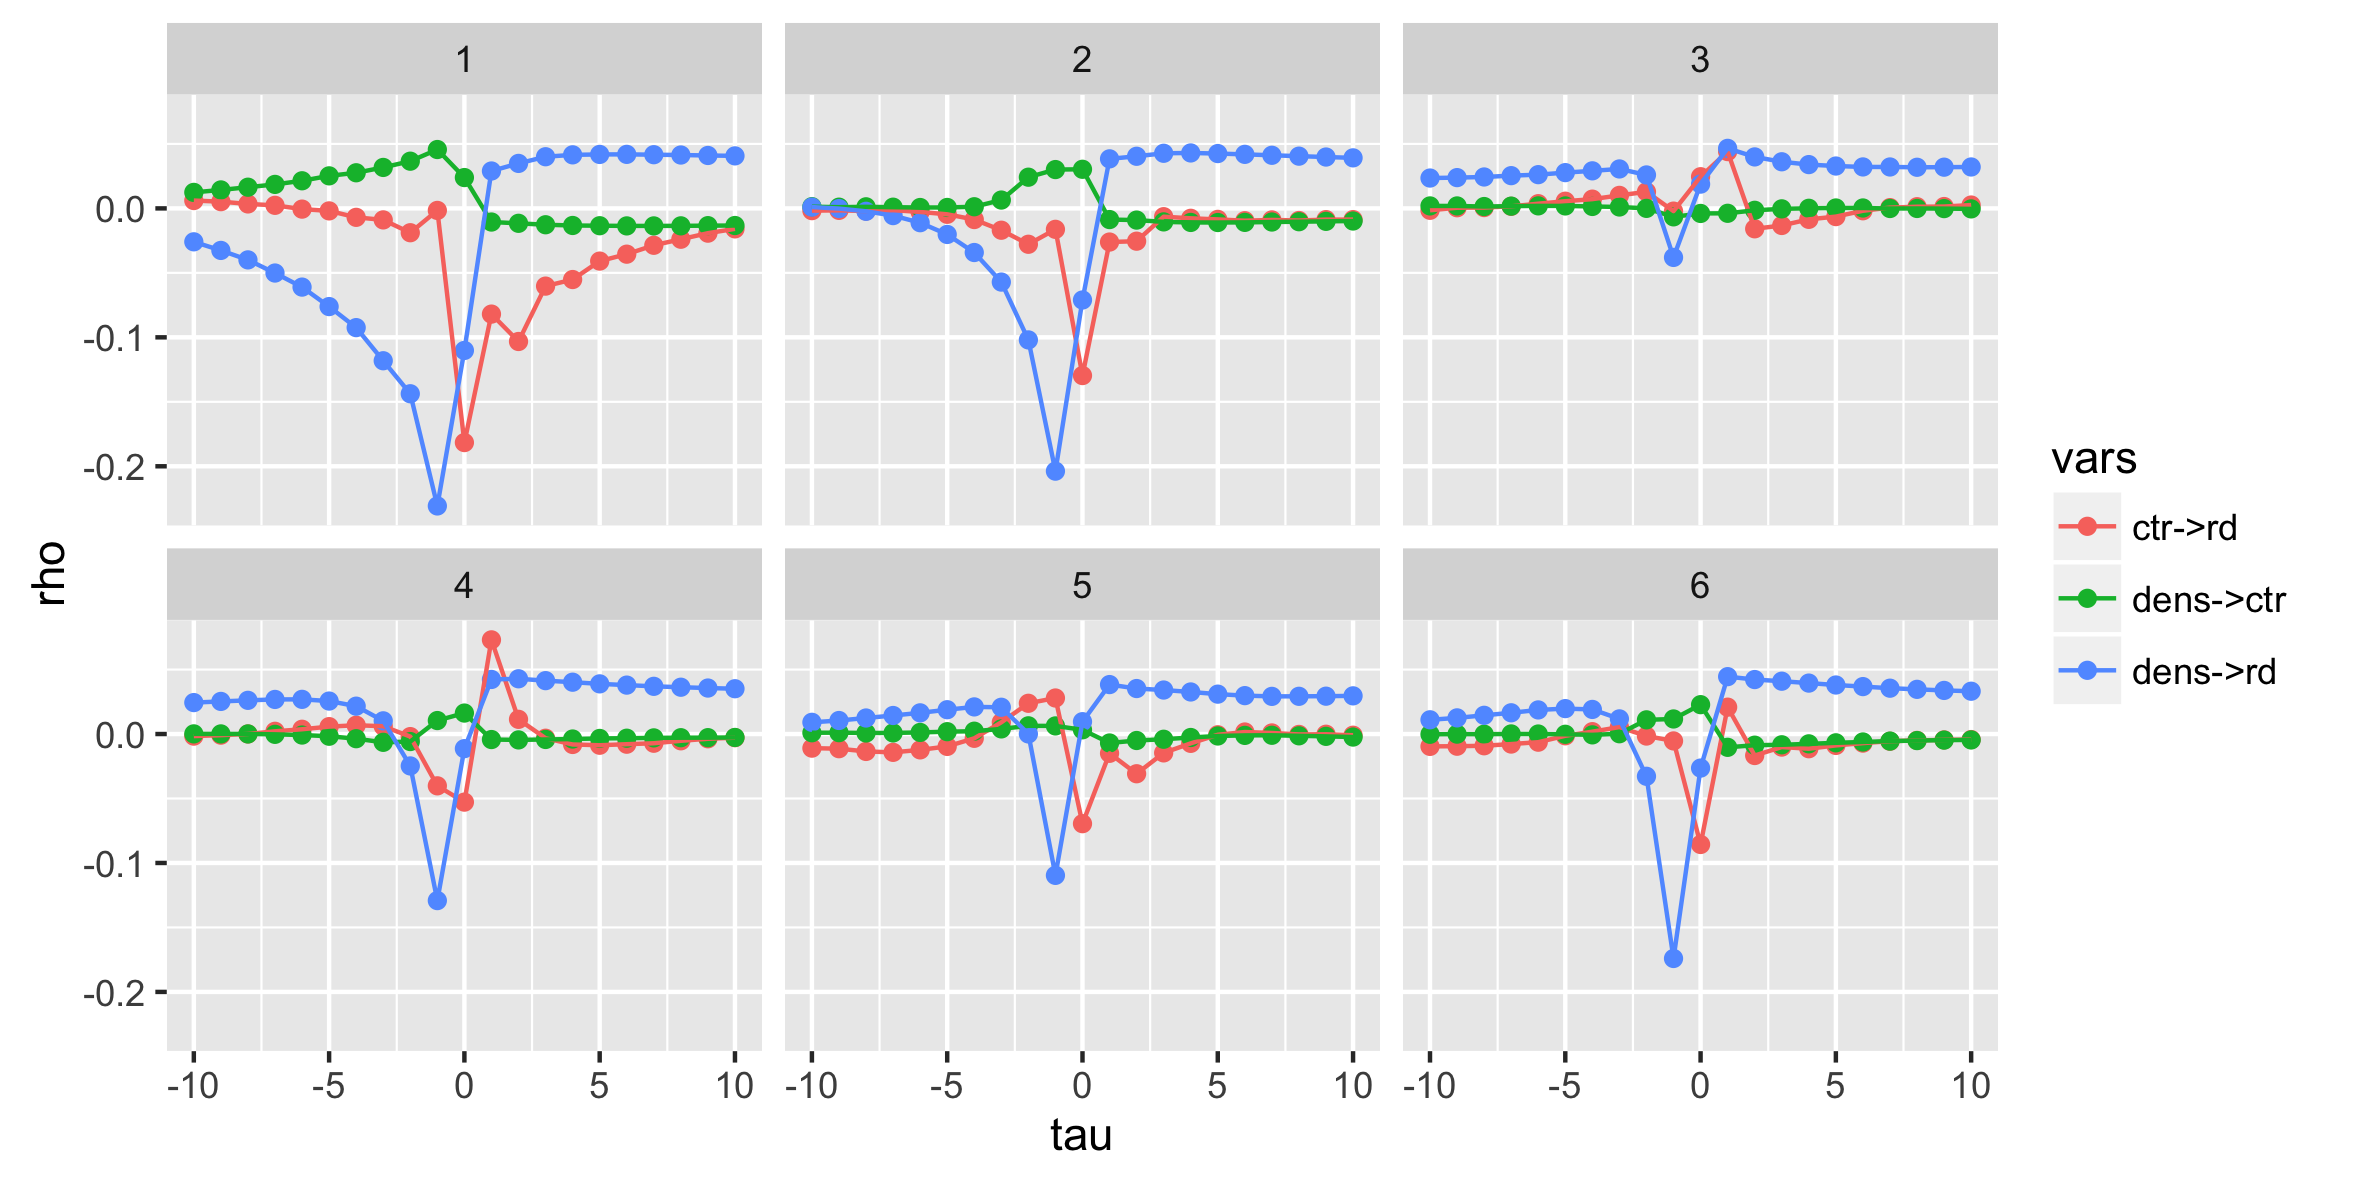
\includegraphics[width=\textwidth]{figures/clusters-centertrajs-facetclust_valuesFALSEtheta2_k6}

\textit{Values of cluster centers in terms of $\rho_{\tau}$}

}

\sframe{Consistence and interpretation of regimes}{

\centering

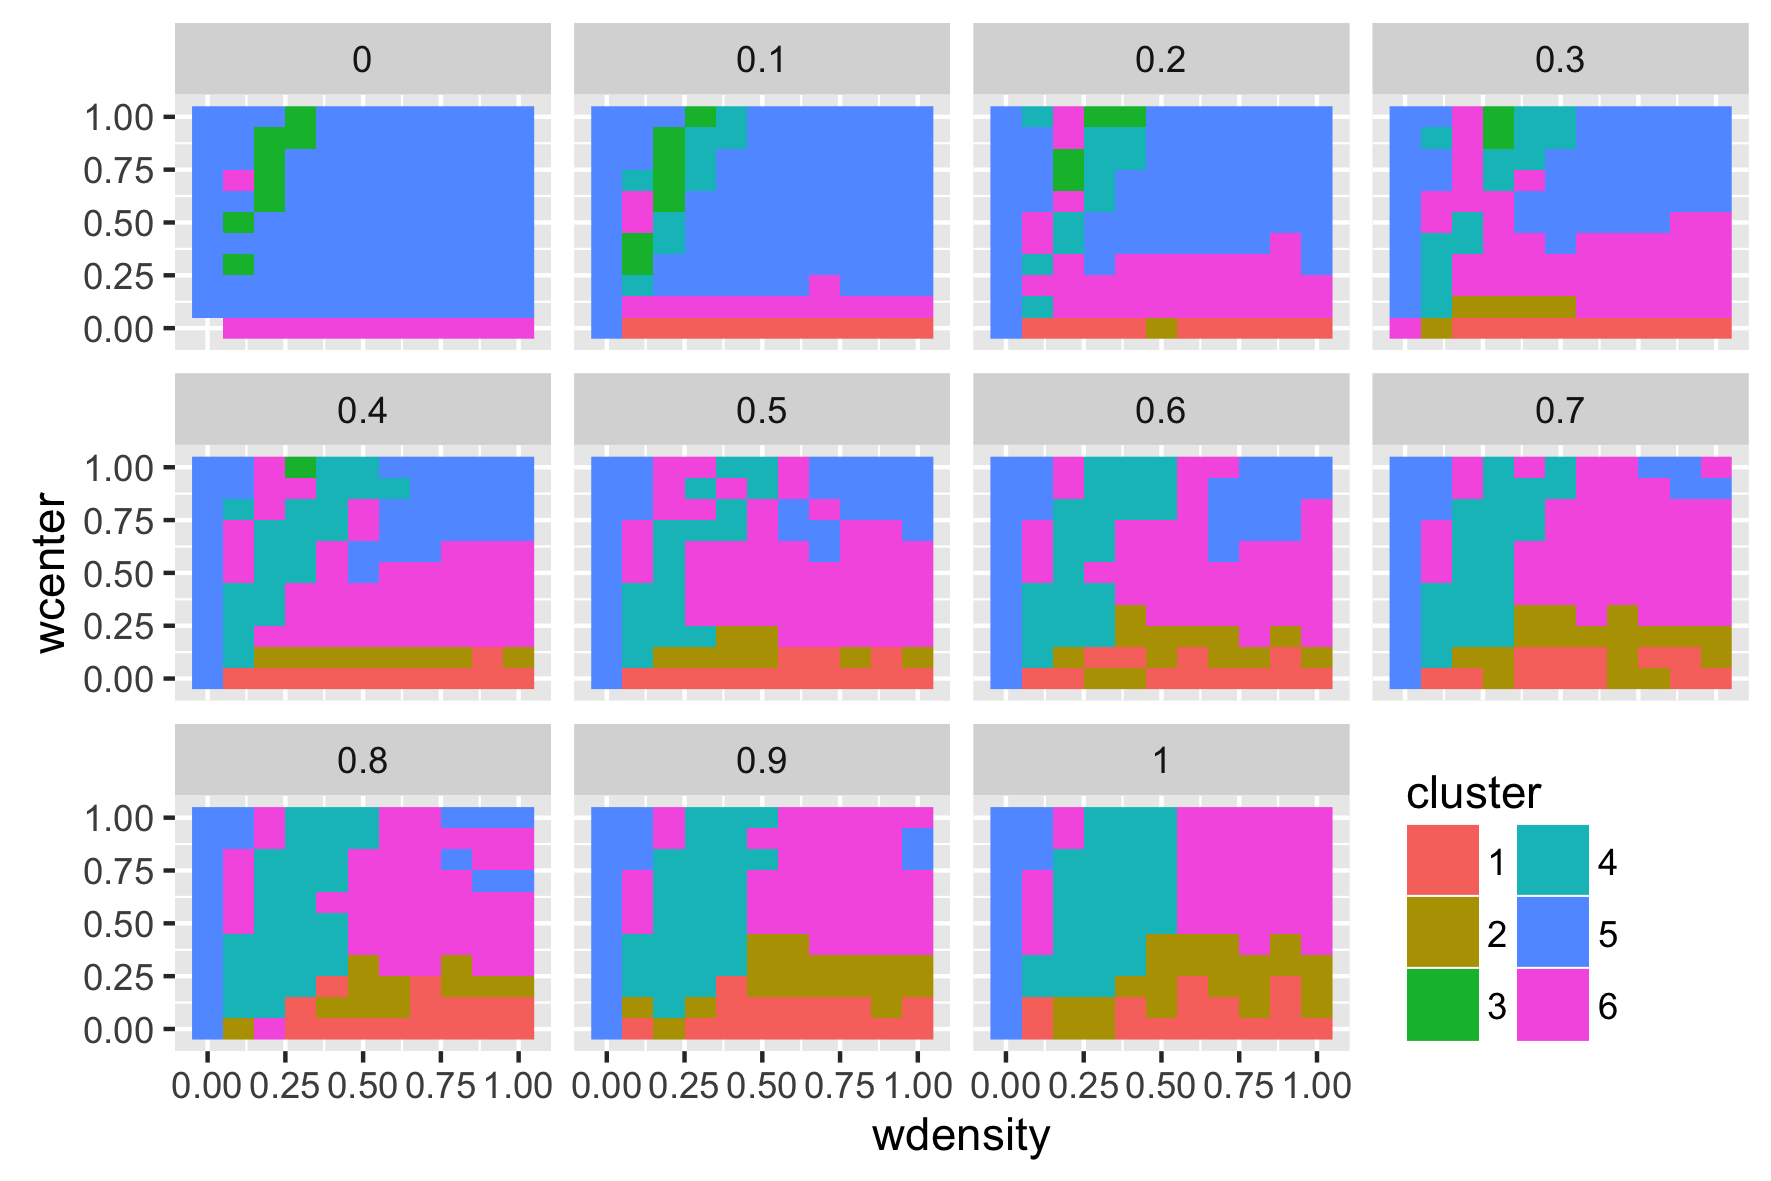
\includegraphics[width=0.9\textwidth]{figures/clusters-paramfacet_valuesFALSEtheta2_k6}

\textit{Position of clusters in the parameter space $w_i$}


}



\sframe{Application: Case study}{

\centering

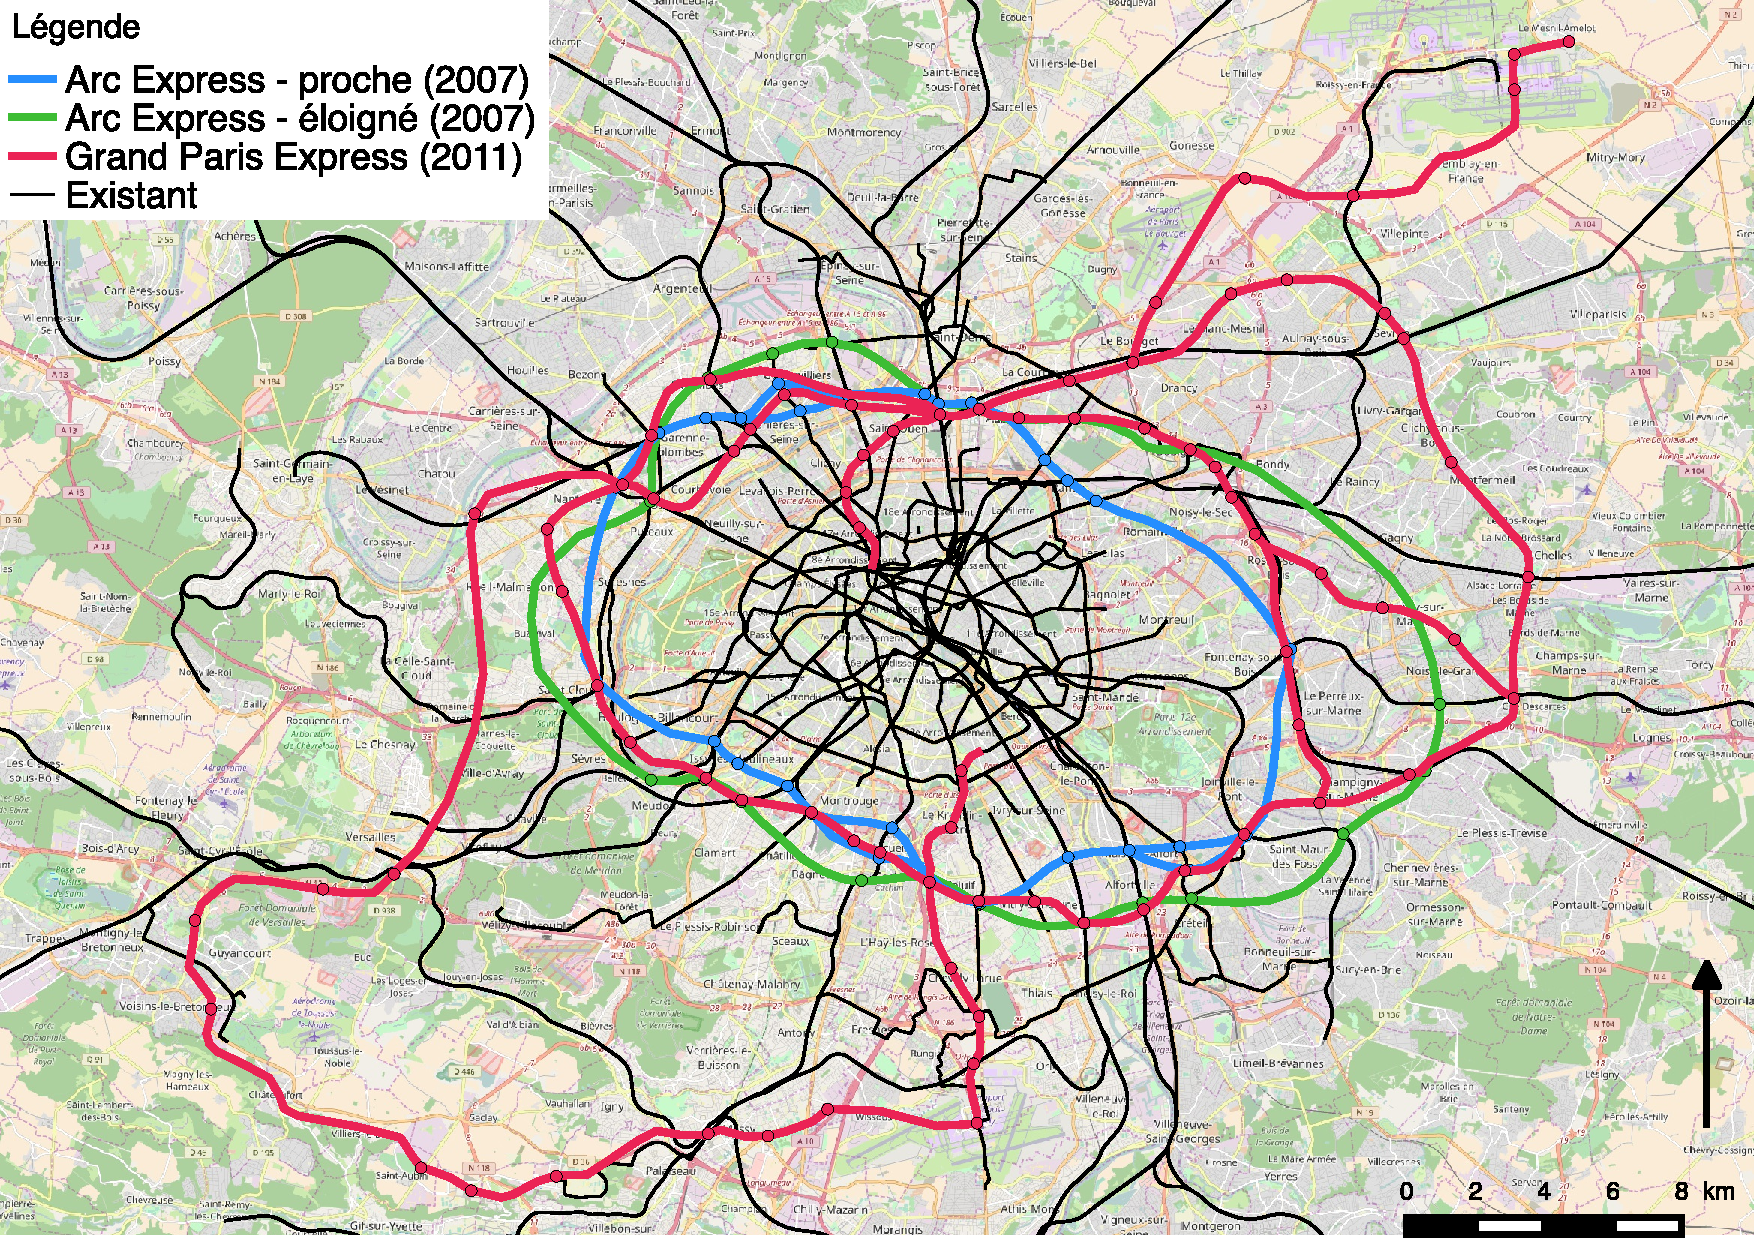
\includegraphics[width=0.8\textwidth]{figures/reseaux}

\medskip

\textit{Successive projects for the Grand Paris new transportation infrastructure}

}


\sframe{Application: Results}{

\centering

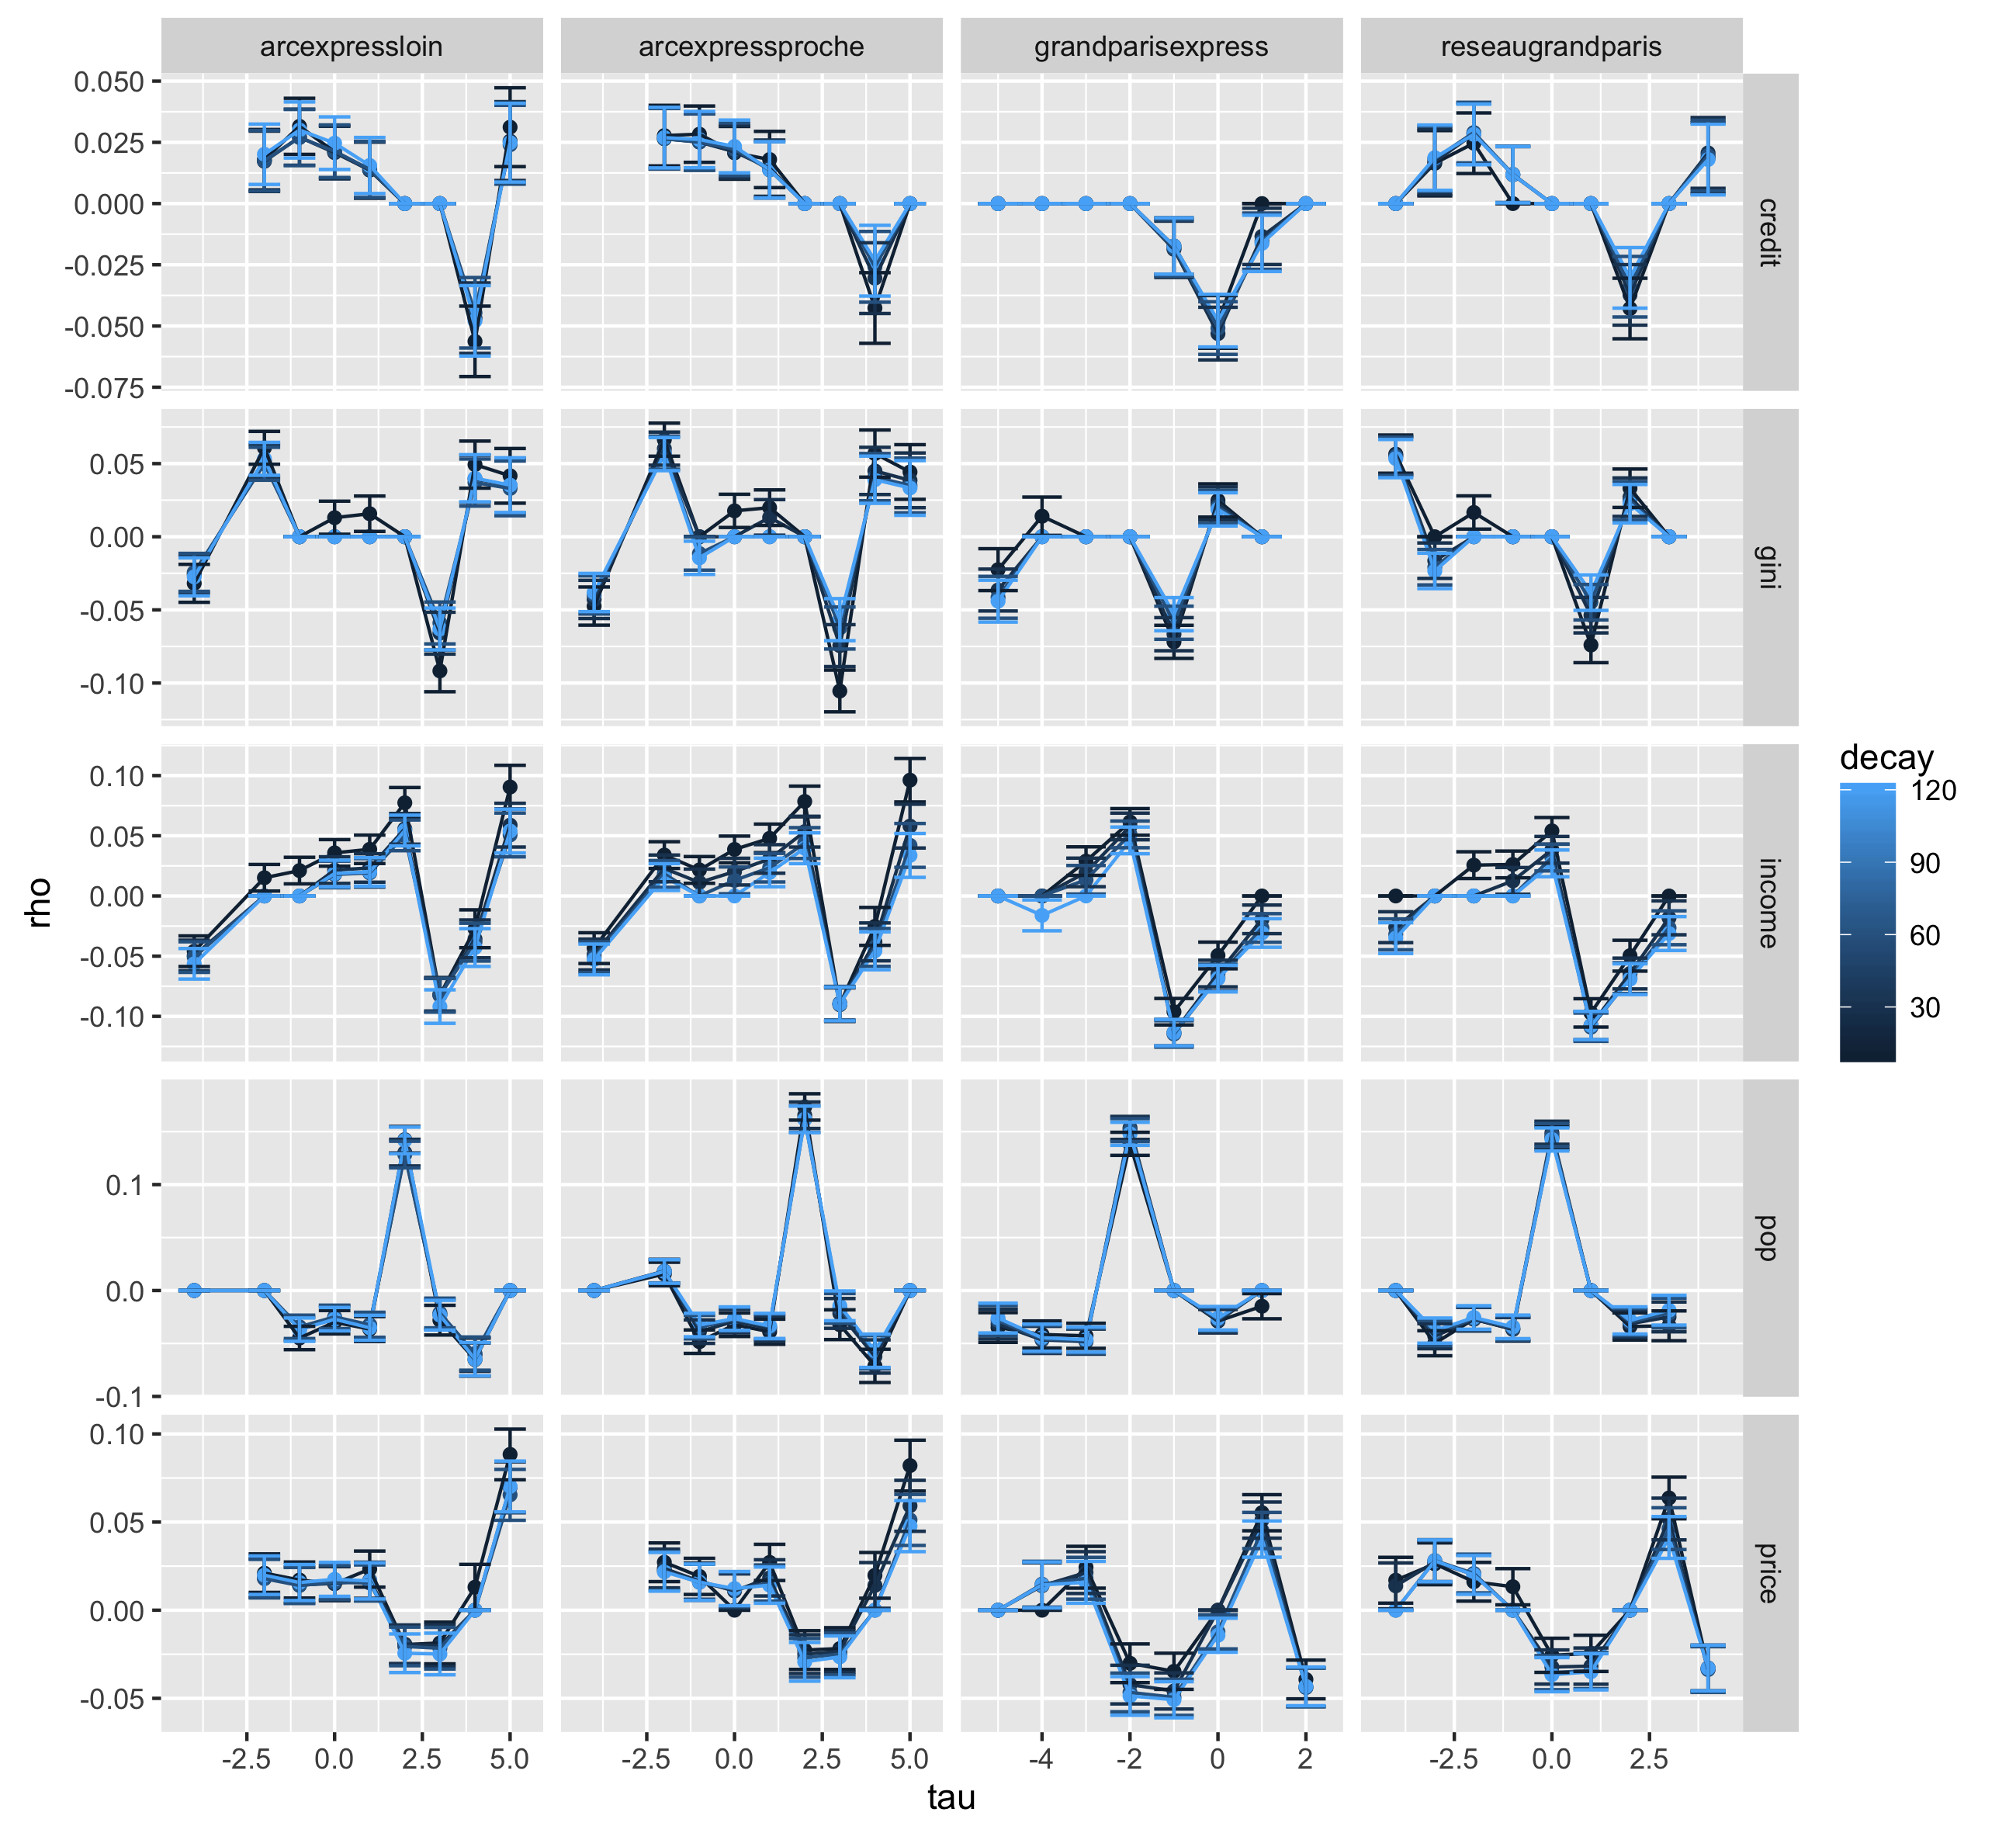
\includegraphics[width=0.62\textwidth]{figures/laggedcorrs_times_allvars}

\textit{Values of $\rho_{\tau}$ for the different projects (columns) and different variables (rows), with accessibility differentials}

}




%%%%%%%%%%%%%%%%%
\section{Discussion}
%%%%%%%%%%%%%%%%%





\sframe{Discussion}{

\justify

\vspace{-1cm}

\textbf{Implications}

$\rightarrow$ 

\bigskip

\textbf{Developments}


$\rightarrow$ 

}




\sframe{Conclusion}{

\justify

$\rightarrow$ 

\bigskip
\bigskip
\bigskip

\footnotesize{ - Code, data and results available at\\ \texttt{https://github.com/JusteRaimbault/CityNetwork}

}

}






\sframe{Reserve slides}{

\centering

\Large

\textbf{Reserve Slides}

}




%%%%%%%%%%%%%%%%%%%%%
\begin{frame}[allowframebreaks]
\frametitle{References}
\bibliographystyle{apalike}
\bibliography{/Users/juste/ComplexSystems/CityNetwork/Biblio/Bibtex/CityNetwork,biblio}
\end{frame}
%%%%%%%%%%%%%%%%%%%%%%%%%%%%









\end{document}







